\chapter{Úvod}
Cílem práce je navrhnout nástroj, který podporuje provádění finanční analýzy podniku. Finanční analýza je v~podnikové sféře soubor činností umožňující zjistit a~vyhodnotit finanční situaci podniku na základě dat o~jeho hospodaření. Její provádění a~zkoumání výsledků je jedním z~předpokladů pro kvalitní a~komplexní vedení podniku. Cílovou skupinu produktu tedy tvoří finanční analytici, manažeři společností i běžní podnikatelé, jimž má usnadnit provádění této činnosti.

Práce obsahuje dva tematické celky. Nejprve bude provedeno shrnutí teorie spojené s~prováděním finanční analýzy -- co je to finanční analýza, jaké jsou její cíle, jaká jsou vstupní data a~co je výstupem, vysvětlení pojmů, používaných metod a~strategií, konstrukcí a~vypočtů jednotlivých ukazatelů finanční analýzy a~intepretací jejich hodnot. 
Druhým tematickým celkem je popis nástroje, který finanční analýzu provádí a~který bude v~rámci této diplomové práce implementován. 

Text práce je členěn do pěti kapitol. Jelikož je finanční analýza poměrně rozsáhlá oblast, celá příští kapitola je věnována prvnímu celku, teorii. 

Ve třetí kapitole jsou ještě před vytvářením návrhu podrobeny testování již existující nástroje, abychom si mohli udělat obrázek o~tom, jak tuto problematiku řešili jiní. Na základě zjištěných poznatků je vypracován návrh programového řešení vlastního nástroje.

Čtvrtá kapitola se zabývá realizací návrhu, implementačními detaily, fungováním nástroje a~také jeho testováním. 

V~závěrečné kapitole jsou shrnuty a~zhodnoceny dosažené výsledky, přínosy této práce a~návrhy na její možná rozšíření.

Pro lepší demonstraci budou v~této práci analyzovány výsledky hospodaření společnosti abc, která se zabývá def. Výkaz zisku a~ztráty a~rozvahu lze najít v~příloze.





























\chapter{Finanční analýza}


\section{Předmět, motivace a~cíle}
Finanční analýza podniku je metoda hodnocení finančního hospodaření podniku, při které se získaná data třídí, agregují, poměřují mezi sebou navzájem, kvantifikují se vztahy mezi nimi, hledají se mezi nimi kauzální souvisloti a~určuje se jejich vývoj. Tím se zvyšuje vypovídací schopnost zpracovávaných dat, zvyšuje se jejich informační hodnota\cite{sedl}.

Motivací je posouzení finanční situace podniku a~její příčiny, do jisté míry i k~predikci stavu podniku v~budoucnu, odhalení důsledků vlastních rozhodnutí, identifikaci slabých míst, plánování, zhodnocení hospodaření, vyvozování závěrů o~vlastnostech podniku, ohodnocení podniku a~vyvozování dalších užitečných informací.

Mimo to se v~praxi lze setkat s~případy, kdy je pro dosažení podnikatelského záměru provedení finanční analýzy nezbytné. Její výsledky jsou směrodatné například při rozhodování banky mezi poskytnutím a~neposkytnutím úvěru, nebo pro vyměření výše úroků.

Při finanční analýze se používají dva navzájem propojené přístupy\cite{kova}:
\begin{enumerate}
	\item kvalitativní (fundamentální) analýza, založená na znalostech souvislostí mezi ekonomickými i mimoekonomickými jevy, zkušenostech odborníků a~na jejich subjektivních odhadech
	\item kvantitativní (technická) analýza, která využívá matematické, statistické a~jiné algoritmizovatelné postupy
\end{enumerate}

V~této práci se budeme zabývat především kvantitativní analýzou právě z~důvodu možnosti její algoritmizace.


\begin{figure}
  \centering
  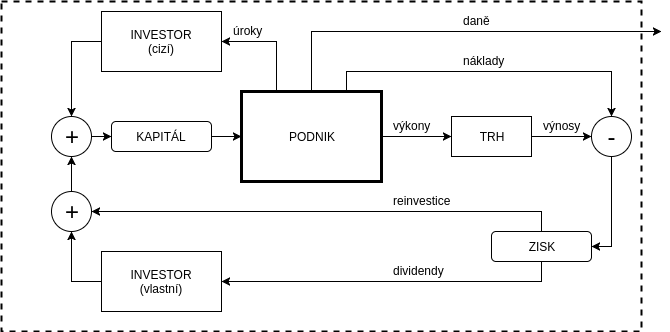
\includegraphics[width=14cm]{img/ccf.png}
  \caption{Schéma finančních toků podniku \cite{sedl}}
  \label{ccf}
\end{figure}

\section{Vstupní data}
Abychom mohli provést finanční analýzu, musíme mít data, ze kterých budeme vycházet. Množina vstupních dat není nijak omezena a~může být vskutku rozsáhlá -- při výpočtu a~odvozování závěrů lze zohlednit nejrůznější faktory, finanční i nefinanční. Pro nás budou však klíčová především data o~vlastním hospodaření podniku, za jejichž evidenci je zodpovědná účetní jednotka podniku, která je v~průběhu roku zapisuje do takzvané účtové osnovy.

\subsubsection{Účtová osnova}
Právnické osoby, fyzické osoby zapsané v~obchodním rejistříku a~některé další subjekty jsou ze zákona o~účetnictví povinny vést podvojné účetnictví, což implikuje povinnost účtovat podle účtové osnovy.
Všechny peněžní toky a~prostředky musí být evidovány na příslušném účtu. Přestože je účtů nespočet, obecně se dají rozdělit do dvou skupin -- rozvahové a~výsledovkové. Tyto subjekty jsou dále povinny každoročně vypracovat a~zveřejnit účetní závěrku, která je tvořena dvěmi finančními výkazy, rozvaha a~výkaz zisku a~ztráty (výsledovka).
Hodnoty jejich položek plynou právě ze sumy hodnot jednotlivých účtů účtové osnovy (rozvahových pro rozvahu, výsledovkových pro výsledovku).

\subsubsection{Výkaz zisku a~ztráty}
Výkaz zisku a~ztráty, také výsledovka, ukazuje, jakého hospodářského výsledku bylo dosaženo v~daném účetním období. Data výsledovky jsou počítány z~dat výsledovkových účtů. Jednotlivé účty jsou kategorizovány podle jejich účelu a~položky výsledovky jsou sumy účtů dané kategorie. Je to jakási agregace záznamů o~pěněžních tocích za celé účetní období, z~nichž každý je buď výnosem nebo nákladem (pozn. není to to samé jako příjmy a~výdaje). Výsledkem hospodaření se rozumí buďto zisk (výnosy převyšují náklady) nebo ztráta (náklady převyšují výnosy).

\subsubsection{Rozvaha}
Také označována termínem bilance. Narozdíl od výkazu zisku a~ztráty jsou při sestavování rozvahy data vázána k~jednomu určitému okamžiku, takzvanému rozvahovému dni, který je posledním dnem účetního období, zpravidla posledním dnem kalendářního roku. Data mají tedy statickou povahu.

Hlavními složkami rozvahy jsou aktiva a~pasiva. Zatímco aktiva představují majetek společnosti (budovy, stroje, materiál, vozidla, \dots, ale i software nebo know-how), pasiva jsou zdrojem krytí těchto aktiv (kapitál). V~průběhu roku se hodnota aktiv a~pasiv liší právě o~hodnotu, o~kterou se liší náklady a~výnosy. Při sestavování závěrky se rozdíl nákladů a~výnosů po zdanění přenese na rozvahový účet (představující pasivum) s~názvem hospodářský výsledek ve schvalovacím řízení, čímž se aktiva a~pasiva vyrovnají. Část zisku musí být investována do fondů (ze zákona, případně stanov společnosti), valná hromada poté rozhodne, co se zbytkem. Může navýšit vlastní jmění podniku nebo zisk rozdělit mezi vlastní investory, což je znázorněno na obrázku \ref{ccf}. Hlavním rozdělením aktiv je na krátkodobá a~dlouhodobá, hlavním rozdělením pasiv je na vlastní a~cizí kapitál.





%-----
\section{Absolutní ukazatele}

\subsection{Horizontální analýza}
Při horizontální analýze je určitá položka (řádek) finančního výkazu porovnávána se stejnou položkou za jiné časové období. Při výpočtu tedy porovnáváme výsledky jedné položky napříč různými obdobími - proto horizontální analýza. U~jednotlivých položek zvlášť je vypočtena absolutní hodnota meziroční změny a~její procentuální vyjádření. Tento postup je proti ostatním velmi ilustrativní, působivý a~přímočarý. 

Při posuzování výsledků by měl analytik zohlednit významné meziroční změny, které mají vliv na výsledek -- změny v~daňové soustavě, podmínek na trhu, změna politické situace, míra inflace a~podobně. Výsledek je běžně interpretován pomocí sloupcového nebo spojnicového grafu. 


\subsection{Vertikální analýza}
Přívlastek vertikální vychází tak jako u~horizontální analýzy ze způsobu zpracování finančních výkazů. Dáváme tak do poměru jednotlivé položky výkazů. Narozdíl od poměrových ukazatelů zmíněných dále se však při vertikální analýze dává do poměru část celku k~celku samotnému. Dalo by se tedy říct, že vyčíslováním podílu vybrané části na celku vertikální analýza popisuje strukturální rozložení sledované entity (například aktiv nebo pasiv či jejich složek). 
Výhodou vertikální analýzy je, že není ovlivněna meziroční inflací a~výsledky se tak dají provnávat s~výsledky za jiné časové období, mimo to i s~výsledky jiných podniků\cite{sedl}.






%-----
\section{Poměrové ukazatele}
Výpočet je opět založen na datech z~rozvahy a~výsledovky. Narozdíl od horizontální a~vertikální analýzy, při kterých je sledován vývoj jedné veličiny v~čase případně vývoj ve vztahu k~určité vztažné veličině (nadřazenému celku), při výpočtu poměrových ukazatelů zkoumáme vztah mezi jednotlivými veličinami navzájem, čímž získáváme zase jinou vypovídací hodnotu.

Existuje několik různých ukazatelů. Různé ukazatele slouží různým účelům, různé společnosti se řídí různými ukazateli. Podle účelu a~povahy ukazatele ho lze zařadit do některé ze skupin soustavy ukazatelů. V~této práci budou zmíněny základní skupiny poměrových ukazatelů -- rentability, likvidity, aktivity a~zadluženosti, v~rámci nichž budou popsány i jednotlivé ukazatele.

Jak plyne z~názvu, při výpočtu hodnoty ukazatele se obecně používá nějakého poměru, tedy zlomku. Možností, které hodnoty dát do poměru, je takřka neomezeně. Nicméně při konstrukci jednotlivých ukazatelů bychom se měli zamyslet nad tím, co při vybraných entitách vlastně vztah vyčísluje -- zda má konkrétní volba význam pro účel analýzy\cite{kisling}.

%-----
\pagebreak
\subsection{Ukazatele rentability}
profitability ratios

Ukazatele rentability (výnosnosti, ziskovosti, návratnosti) patří v~praxi mezi nejsledovanější ukazatele. Vyjadřují míru efektivity hospodaření podniku poměřením výsledku hospodaření se zdroji, které byly na hospodaření vynaloženy.

$$\zl{výsledek hospodaření}{zdroje}$$

Ukazatele rentability jsou mezivýkazovými ukazateli, což znamená, že jsou při jejich výpočtu použity hodnoty z~výsledovky i rozvahy. Jednotlivé ukazatele rentability se liší především tím, co je chápáno pod pojmem zdroje ve jmenovateli\cite{mendelu}. Podle volby jmenovatele je vytvořeno také následující rozdělení ukazatelů rentability. 

V~rámci jednoho ukazatele však existuje několik dalších variant výpočtu. Ty se vzájemně liší složkou v~čitateli, která zachycuje výsledek hospodaření (zisk) v~rozdílných fazích -- před nebo po zdanění, odečtení úroků, provedení odpisů a~amortizace. Do čitatele může být dosazen i jiný ukazatel firemní výkonosti, jako například provozní cashflow. Volíme takové hodnoty, které mají pro danou situaci největší vypovídací hodnotu.

\begin{itemize}
\item EAT -- earnings after taxes, čistý zisk -- zisk po zdanění, zúročení, odpisech a~amortizaci

\item EBT -- earnings before taxes, hrubý zisk -- zisk před zdaněním, t.j. po odečtení úroků, odpisech a~amortizaci

\item EBIT -- earnings before interest and taxes, provozní zisk -- zisk před zdaněním a~zúročením. Uzití této hodnoty je vhodné například při srovnávání dvou podniků s~různou výší daně z~příjmu a~různou kapitálovou strukturou

\item EBITDA -- earnings before interest, taxes, depreciation and amortization -- zisk před zdaněním, úroky, odpisy a~amortizací

\item NOPAT = EBIT$*(1-t)$, kde $t$ je sazba daně z~příjmů  -- zdaněný (čistý) zisk bez odečtení úroků, t.j. kolik by dělal čistý zisk, kdyby podnik nemusel platit úroky (kdyby nečerpal žádný úvěr)
\end{itemize}


\begin{figure}
  \centering
  
\includegraphics[width=10cm]{img/zisk.png}
  \caption{Grafická intepretace jednotlivých druhů zisku}
\end{figure}

%-----
\subsubsection{ROA -- rentabilita aktiv}
return on assets

ROA je ukazatel, který do jmenovatele dosazuje celkový objem aktiv (potažmo pasiv, jelikož jsou jimi kryta). Při výpočtu se tedy nebere ohled na to, zda jsou aktiva vlastní nebo cizí, dlouhodobá nebo krátkodobá. Tím vyjadřuje, jak efektivně dokáže podnik naložit s~aktivy, které se do něj vloží (odtud zřejmě plyne označení produkční síla nebo výkonnost podniku).

Nejčastějšími variantami uváděnými v~literatuře jsou ty, které mají v~čitateli hodnotu EBIT, tedy zisk před odečtením nákladových úroků (rentabilita celkových aktiv by neměla brát v~potaz původ zdrojů) a~zdaněním. Tato volba nám zároveň umožňuje porovnat podniky s~rozdílnými zdroji financování a~různým daňovým zatížením.

$$\vz{ROA}{EBIT}{A} \scite{sedl}$$

Další používanou variantou je s~hodnotou NOPAT v~čitateli. Výsledkem je rentabilita, která by plynula z~čistého zisku, pokud by byly veškeré zdroje financování vlastní. Dochází zde k~fiktivnímu zdanění úroků, jelikož EBIT$*(1-t)$ se dá zapsat také jako EAT$+$Ú$*(1-t)$.

$$\vz{ROA}{EBIT $*(1-t)$}{A} \scite{sedl}$$ 


%-----
\subsubsection{ROE -- rentabilita vlastního kapitálu}
return on equity

ROE do jmenovatelele dosazuje hodnotu vlastního kapitálu, čímž vyjadřuje míru jeho zhodncení. Jinými slovy udává, kolik korun zisku připadá na 1 korunu vlastního kapitálu. Pro vlastníky (akcionáře, společníky a~další investory) podniku je jedním z~klíčových ukazatelů, neboť pomocí něj mohou zjistit, zda jimi vložený kapitál přináší výnos odpovídající velikosti jejich investičního rizika\cite{sedl}.

Investor by se měl také zajímat, zda je procentuální hodnota ROE vyšší než bezriziková úroková míra (úroková sazba státních dluhopisů), v~praxi spíše vyšší než nejvyšší úroková sazba nabízená bankami. Pokud by byla nižší, obnos investovaný do podniku by mohl raději vložit do banky a~téměř bez námahy a~bez rizika dosáhnout většího výnosu.

Výpočet má pochopitelně smysl zejména s~čistým ziskem (EAT) v~čitateli, avšak ve jmenovateli můžeme uvažovat nad odečtením fondů, ze kterých investor ve výsledku těžit nebude.

$$\vz{ROE}{čistý zisk}{vlastní kapitál} \scite{sedl}$$ 


%-----
\subsubsection{ROS -- rentabilita tržeb}
return on sales

V~praxi velmi často používaný ukazatel. Poměřuje zisk podniku a~tržby (tržby za prodej zboží, výrobků a~provedení výkonů), tedy kolik procent tržeb tvoří zisk.

Pokud by byla výsledkem relativně malá, dlouhodobě klesající hodnota (např. 2\%), je vhodné zpozornit. Pokud by došlo k~náhlému poklesu tržeb při zachování nákladů (což je běžné), je zřejmé, že se podnik dostane do finančních potíží. Stejnětak se může dostat do potíží při zvýšení nákladů (zdražení materiálu, energií, pracovní síly) se současným zachováním objemu tržeb (zvýšení nákladů se však na tržby zpravidla promítne). 
V~čitateli se nejčastěji používá hodnota EBIT nebo EAT

$$\vz{ROS}{EBIT}{tržby} \scite{sedl} \hspace{2cm} \vz{ROS}{EAT}{tržby} \scite{sedl}$$ 

%-----
\subsubsection{ROI -- rentabilita investice}
return on investment

Další z~často používaných ukazatelů. Jak napovídá název, ukazatel vyjadřuje rentabilitu spíše z~pohledu konkrétního investičního projektu, z~výše sumy investic provedených během vymezeného období, nežli z~celopodnikového pohledu. Oba přístupy by pojednávaly o~tom samém v~případě, že by se jednalo o~investici do koupi podniku. Rentabilita této investice by pak byla stejná jako rentabilita vlastního kapitálu, v~případě nezadluženého podniku i stejná jako rentabilita celého podniku.

$$\vz{ROI}{výnos investice}{náklady na investici} \scite{sedl} $$ 

%-----
\subsubsection{Některé další ukazatele rentability:}
\begin{itemize}
\item{ROC -- rentabilita nákladů} -- return on costs
\item{ROCE -- rentabilita dlouhodobě investovaného kapitálu} -- return on capital employed
\end{itemize}







%-----
\subsection{Ukazatele likvidity}
Pojem likvidita bývá nesprávně zaměňován s~úzce souvisejícími pojmy likvidnost a~solventnost. Likvidnost je vlastnost jednotlivých složek aktiv podniku vyjadřující schopnost přeměny těchto složek v~peněžní prostředky v~co nejkratším čase a~s~minimálními ztrátami\cite{nyvlt}. Přeměnou můžeme rozumět například prodej zásob nebo inkasování pohledávek. 

Solventnost neboli platební schopnost je definována jako schopnost subjektu, v~našem případě podniku, včas splácet své finanční závazky. Má-li být podnik solventní, musí kromě stálého generování zisku také zajistit, aby byla část aktiv vázána ve formě, kterou může uhradit své závazky.

Likvidita podniku dává tyto pojmy do souvislosti -- ukazatele likvidity vyjadřují schopnost podniku přeměnit vybraná aktiva na peněžní prostředky (využít jejich likvidnosti) za účelem včasného uhrazení všech splatných závazků (a tím pádem být dočasně solventní)\cite{schol}. Proto bývají také označovány jako ukazatele platební schopnosti.

Všechny ukazatele likvidity se počítají jako poměr toho, čím je možné platit (disponibilní prostředky), k~tomu, co se musí zaplatit. Disponibilními prostředky můžeme přitom chápat různou množinu aktiv. Je samozřejmě nesmysl, aby byla zahrnuta ta aktiva, jejichž ztráta by ohrozila chod podniku.

%-----
\pagebreak
\subsubsection{Běžná likvidita (likvidita III. stupně)} 
CR - Current Ratio

Poměr ukazuje, kolikrát pokrývají oběžná aktiva krátkodobé závazky, jinými slovy, kolikrát je podnik schopen uhradit své krátkodobé závazky z~peněžních prostředků, které by získal přeměnou z~oběžných aktiv.

Uváděná optimální hodnota se v~literaturách různí, zřejmě se bude lišit i v~závisloti na typu podniku. Hodnota ukazatele by určitě neměla být menší než 1, což by znamenalo nutnost financovat závazky z~dlouhodobých zdrojů financování a~jinými nevhodnými způsoby. Také berme v~potaz, že po pokrytí závazků by měly zbýt prostředky pro další činnost podniku.
Optimální hodnota uvedená v~preferovaném zdroji je CR$\geq 1.5$, ale obecně lze tvrdit, že čím stabilnější jsou příjmy a~čím jistější jsou zdroje těchto příjmů, tím více se může hodnota běžné likvidity blížit jedné\cite{businessvize_bez_likv}.

$$\vz{CR}{oběžná aktiva}{krátkodobé závazky} \scite{sedl}$$

%-----
\subsubsection{Pohotová likvidita (likvidita II. stupně)} 
QAR - Quick Asset Ratio

Pokud bychom zkoumali strukturu oběžných aktiv, zjistili bychom, že se likvidnost jednotlivých složek liší. Výpočet běžné likvidity zahrnuje i zásoby, nicméně ty při výpočtu pohotové likvidity nejsou zahrnuty, jelikož většinou bývají nezbytné pro zachování chodu podniku a~navíc jejich likvidnost nemusí být dostačující.
V~čitateli tak zbude součet objemu peněžních prostředků, ekvivalentů a~pohledávek. Pro zpřesnění výsledku je vhodné odečíst nedobytné pohledávky.
Dá se předpokládat, že podniky z~oblasti služeb nebudou mít v~zásobách mnoho aktiv a~proto se bude hodnota ukazatele blížit hodnotě běžné likvidity. U~výrobních podniků se naopak tyto dvě hodnoty budou spíše lišit.

$$\vz{QAR}{oběžná aktiva $-$ zásoby}{krátkodobé závazky} \scite{sedl}$$

%-----
\subsubsection{Hotovostní likvidita (likvidita I. stupně)}
CPR - Cash Position Ratio

Při výpočtu hotovostní likvidity dosazujeme do čitatele součet jen těch nejlikvidnější složek oběžných aktiv, kterými jsou pěněžní prostředky (peníze v~hotovosti a~na běžných účtech) a~jejich ekvivalenty (například šeky nebo obchdovatlné cenné papíry).
Přestože tento ukazatel nejlépe vypovídá o~platební schopnosti podniku k~určitému datu, nebere v~potaz strkuturu krátkodobých závazků, především z~pohledu jejich skutečné splatnosti\cite{mendelu}. Pokud bychom chtěli tuto skutečnost zohlednit, měli bychom do jmenovatele zahrnout pouze okamžitě splatné závazky. Taková varianta bývá označována jako okamžitá likvidita.


$$\vz{CPR}{peněžní prostředky $+$ ekvivalenty}{krátkodobé závazky} \scite{sedl}$$








%-----
\subsection{Ukazatele aktivity}
Další z~mezivýkazových ukazatelů -- vstupními daty jsou položky jak z~výkazu zisku a~ztrát tak z~rozvahy. Ukazatele aktivity vyjadřují, jak efektivně podnik nakládá se svými aktivy. Pokud jich vlastní více, než je nutné, vznikají zbytečné náklady a~dochází ke snižení zisku. Jestliže jich má nedostatek, přichází o~výnosy z~potenciálních zakázek, o~které se kvůli nedostatku aktiv nemůže ucházet.

Výsledkem je hodnota udávající rychlost nebo dobu obratu. Rychlost obratu vyjadřuje, kolikrát se určitá složka aktiv přemění za sledované období na peněžní prostředky. Doba obratu nám říká, jak dlouho trvá přeměna.

Pokud známe hodnotu rychlosti obratu sledovaných aktiv X, dobu obratu X (výsledkem budou dny) vypočítáme jednoduše jako 

$$\vz{doba obratu}{365}{rychlost obratu X}$$


%-----
\subsubsection{Obrat celkových aktiv}
total assets turnover

Udává, kolikrát se obrátí celková aktiva za sledované časové období. Nevýhodou tohoto a~některých dalších ukazatelů je povaha vstupních veličin: tržby jsou zachyceny jejich sumou za celé období, kdežto hodnota aktiv se vztahuje ke konkrétnímu časovému okamžiku, kdy byla rozvaha vytvořena. Přesnějšího výsledku by se dalo dosáhnout použitím průměrné hodnoty sledovaných aktiv. 

$$\vz{obrat celkových aktiv}{tržby}{celková aktiva} \scite{mendelu}$$

%-----
\subsubsection{Obrat stálých aktiv}
fixed assets turnover

Stálá aktiva jsou taková, která slouží podniku déle než jeden rok a~jsou spotřebovávána postupně, nikoliv jednorázově. Konkrétně je to součet dlouhodobého hmotného, nehmotného a~finančního majetku, t.j. například budovy, pozemky, vozidla, stroje, software, know-how a~mnoho dalších.

Ukazatel potom vyjadřuje míru využití těchto aktiv. Pokud při analýze vyjde hodnota nižší, než je průměr v~odvětví, může to znamenat nedostatečné využití stávajících fixních (dlouhodobých) aktiv a~manažeři by tak měli zvážit, jak jejich využití zefektivnit namísto investování do aktiv nových.

$$\vz{obrat stálých aktiv}{tržby}{dlouhodobý hmotný majetek} \scite{mendelu}$$

%-----
\subsubsection{Obrat zásob}
inventory turnover

Říká, kolikrát je za sledované období položka zásob prodána a~opět naskladněna.

Při použití tohoto ukazatele je nutné si uvědomit, že tržby vyjadřují tržní hodnotu (za kolik se prodalo), kdežto hodnota zásob bývá vyjádřena jejich pořizovací cenou (za kolik se nakoupilo). Přesnějšího výsledku obratovosti může být dosaženo umístěním nákladů na prodané zboží do čitatele namísto tržeb.

Ukazatel pro zásoby výrobků nebo zboží je rovněž ukazatelem likvidnosti těchto zásob (udává, jak dlouho trvá přeměna zásob na finanční prostředky).

$$\vz{obrat zásob}{tržby}{zásoby} \scite{mendelu}$$


%-----
\subsubsection{Doba obratu pohledávek}
V~tomto případě je směrodatnější spíše doba trvání pohledávky než počet obratů pohledávek. Doba se vypočítá jako poměr průměrného stavu pohledávek k~průměrné denní tržbě na obchodní úvěr (fakturu, \uv{sekeru}).

Hodnota ukazatele dlouhodobě vyšší než hodnota stanovená platebními podmínkami pro klienta může znamenat problémové portfolio odběratelů, kteří nejsou schopni plnit své závazky včas.

$$\vz{doba obratu pohledávek}{prům. stav pohledávek}{prům. denní tržby} \scite{mendelu}$$

\subsubsection{Doba obratu závazků}
Průměrná doba odkladu plnění závazků. Nabízí se porovnání s~dobou obratu pohledávky. 





%-----
\subsection{Ukazatele zadluženosti}

Zadluženost podniku souvísí s~velikostí podílu cizích zdrojů na všech zdrojích financování podniku, jelikož cizí zdroje pro podnik zpravidla znamenají dluh, závazek. Měří tedy dopady financování cizími zdroji. Využití cizích zdrojů se vyplácí, dokud zajistí výnos vyšší, než jsou náklady na tyto zdroje -- úroky.

V~praxi se běžně nesetkáme s~většími podniky, které by byly financovány výhradně z~vlastních nebo výhradně z~cizích zdrojů, jsou tedy do jisté míry zadluženy. Zadluženost obecně není negativní charakteristikou -- využití cizích zdrojů vede k~zesílení tzv. finančního pákového efektu, který pozitivně přispívá k~rentabilitě vlastního kapitálu\cite{kisling}. S~rostoucím procentem vyjadřujícím zadluženost však roste i riziko věřitelů. Čím vyšší bude riziko věřitelů, tím obtížněji bude podnik další cizí zdroje získávat a~tím nevýhodnější budou podmínky jeho poskytnutí\cite{mendelu}. Jedním z~důležitých cílů finanční analýzy je nalezení ideální míry zadluženosti respektive ideálního rozložení finanční struktury. Vzhledem k~poměrně rozšířenému leasingovému financování zmíním, že by bylo vhodné takto pořízený majetek zohlednit a~přičíst k~cizímu kapitálu, má-li významnější objem.

\begin{figure}
  \centering
  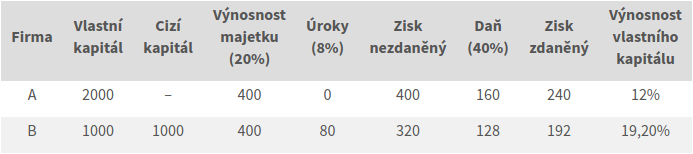
\includegraphics[width=15cm]{img/tab.png}
  \caption{Srovnání výnosnosti při různém poměru vlastního a~cízího kapitálu}
\end{figure}

% \begin{figure}
%   \centering
%   \begin{tabular}{ C{11mm}  C{13mm}  C{12mm}  C{11mm}  C{11mm}  C{18mm}  C{11mm}  C{11mm}  C{12mm} }
%     \hline
%     Firma & Vlastní kapitál & Cizí kapitál & ROA (20\%) & Úroky (8\%) & Zisk nezdaněný & Daň (40\%) & Zisk čistý & ROE \\ 
%     \hline
%     A & 2000 & -- & 400 & 0 & 400 & 160 & 240 & 12\% \\
%     B & 1000 & 1000 & 400 & 80 & 320 & 128 & 192 & 19,20\% \\
%     \hline
%   \end{tabular}
%   \caption{Srovnání výnosnosti při různém poměru vlastního a~cízího kapitálu}
% \end{figure}


%-----
\subsubsection{Celková zadluženost}
debt ratio

Základním ukazatelem zadluženosti je celková zadluženost jako podíl cizího kapitálu na celkových aktivech. S~rostoucí hodnotou tohoto ukazatele roste i riziko věřitelů a~cena za cizí kapitál (výše úroků). Věřitelé preferují nižší hodnoty -- v~případě likvidace podniku mohou být pohledávky (nejen) věřitelů uhrazeny z~vlastního kapitálu podniku (takzvaný finanční polštář).
Z~hlediska vlastníků akcií jsou vysoké hodnoty ukazatele příznivé, dokud podnik dosahuje vyššího procenta rentability než je procento úroku na cizí kapitál, což znamená, že výsledné zhodnocení kapitálu je vyšší než jeho pořizovací cena\cite{such}. 

$$\vz{DR}{cizí kapitál}{celková aktiva} \scite{sedl}$$

\vspace{3mm}
Doplňkovým ukazatelem k~celkové zadluženosti je ukazatel poměru vlastního kapitálu (equity ratio, ER). Jejich součet by měl být DR$+$ER$
\doteq 1$

$$\vz{ER}{vlastní kapitál}{celková aktiva} \scite{sedl}$$

%-----
\subsubsection{Koeficient (míra) zadluženosti}
debt to equity ratio

Dá se spočítat jako poměr hodnoty cízího kapitálu k~hodnotě vlastního. Stejný výsledek bychom získali poměrem předchozích dvou ukazatelů. V~případě, že podnik využívá ve větším objemu leasingového financování, je vhodné tuto skutečnost zohlednit přičtením objemu k~cizímu kapitálu. 

$$\vz{DtE}{cizí kapitál}{vlastní kapitál} \scite{sedl}$$

\vspace{3mm}
Ve finanční analýze se používá i převrácená hodnota ukazatele, která by se dala nazvat jako míra finanční samostatnosti podniku.

%-----
\subsubsection{Úrokové krytí}
interest coverage

Ukazatel vyjadřuje, kolikrát podnik pokryje úroky plynoucí ze závazků věřitelům poté, co uhradí všechny náklady na provoz (tzn. z~provozního zisku). Dá se tedy chápat jako dopad zadlužení na zisk. Obecně platí, že čím vyšší je jeho hodnota, tím lépe pro podnik. Pokud by byla hodnota IC$<1$, znamená to, že podnik hospodaří se ztrátou (není schopen ani pokrýt úroky). Pokud by vyšla hodnota ukazatele IC$=1$, znamená to, že se veškerý zisk použije k~uhrazení úroků za vypůjčený kapitál a~k~vyplacení vlastních investorů nebo k~reinvestici do kapitálu nezbudou žádné prostředky.

$$\vz{IC}{EBIT}{nákladové úroky} \scite{sedl}$$








\subsection{Další ukazatele}

\subsubsection{IRR -- vnitřní výnosové procento}
internal rate of return

Vnitřní výnosové procento vyjadřuje míru výnosnosti investice, tedy ROI, se současným zohledněním proměnné hodnoty peněz v~čase (diskontace). Ve světě patří spolu s~NPV (net present value, čistá současná hodnota) mezi nejpoužívanější ukazatele pro zhodnocení a~výběr investice. Podle průzkumu VŠE je v~ČR preferován spíše ukazatel doby návratnosti investice\cite{businessvize_irr}.

NPV slouží k~přiblížení, kolik peněz nám projekt, jehož investování zvažujeme, za sledované období přinese nebo sebere. Nebere přitom nijak v~úvahu výnosy a~náklady nebo hodnotu společnosti, proto je nevhodný pro strategické projekty. Nevýhodou NPV a~tím pádem i IRR je nutnost odhadu nejen budoucích finančních toků, které sledovaný projekt přinese, ale také výše diskontu. Odhad hodnoty lze zpřesnit různými technikami (viz doporučená literatura). Důležitá je také odhadovaná doba životnosti projektu, přidáním nebo odebráním jednoho období se může změnit ztráta na zisk i opačně.

Nejprve si uvedeme vzorec pro výpočet čisté současné hodnoty: 
\\($r=$diskont, $t=$pořadí období, $CF_t$=suma toků v~období, $IN=$vstupní investice)
$$NPV=\sum\limits_{t=0}^{n} \dfrac{CF_t}{(1+r)^t} = \sum\limits_{t=1}^{n} \dfrac{CF_t}{(1+r)^t} - IN\scite{businessvize_irr}$$

Matematicky lze IRR vyjádřit hodnotou diskontní sazby, při které je čistá současná hodnota (NPV) rovna nule. Dostáváme tedy následující vzorec:
$$\sum\limits_{t=1}^{n} \dfrac{CF_t}{(1+IRR)^t} - IN = 0 \scite{businessvize_irr}$$

Z~uvedeného vzorce lze usoudit, že nalezení hodnoty analytickým řešením není triviální. Rovnice se řeší numericky, iterativními výpočty.





































\chapter{Návrh řešení}



\section{Existující software}
Před návrhem řešení bylo vhodné prozkoumat existující řešení. Plné verze nástrojů pro tyto účely bývají zpoplatněny, závěry jsou tedy vyvozeny ze zkušebních verzí, pochopitelně s~omezenou funkcionalitou, případně z~náhledů a~uživatelských dokumentací software.

Všechny testované nástroje jsou ve formě desktopových aplikací určených pouze pro platformu Windows.

\subsubsection{FAF -- Finanční analýza firmy}
Software nelze bez zakoupení jakkoliv používat, nicméně na webových stránkách je dostupné instruktážní video a~uživtelská přiručka popisující jak nástroj vypadá, jak se s~ním pracuje a~co všechno dokáže. Uživatelské rozhraní vypadá na první pohled zastarale, to ale nijak neubírá na přehlednosti.

Uživatelské rozhraní kromě grafů využívá také stupnic, na které umisťuje ukazatele. Je zde obrazovka \uv{rating}, což jsou různé ukazatele, každý z~ukazatelů je zobrazen za různá časová období a~v~konkrétním časové období na stupnici od 1 do 10. Všechny ukazatele pohromadě lze zobrazit v~tabulce pro jedno časové období.

Ukazatele jsou i na obrazovce s~trendy, ta mimo ukazatele obsahuje i trendy položek výkazu zisku a~ztráty a~rozvahy. Je zde také zobrazen seznam rizikových faktorů. Ty se od ukazatelů liší tím, že jsou buďto v~pořádku nebo ne, nic mezi tím (např. skutečnost, že podnik hospodaří se ztrátou).

Nástroj dále umožňuje vertikální analýzu, horizontální analýzu, analýzu cash flow a~výpočet hodnoty firmy.

Funkcionalita, která mě nejvíce zaujala, je nazvaná \uv{co když}. Spočívá v~umožnění uživateli jednoduše manipulovat se vstupními daty analýzy a~zároveň sledovat, jaký dopad by se měla tato změna na hodnotu ukazatelů.

Hodnoty z~ výkazu zisku a~ztráty a~rozvahy jsou zadávány do tabulky. Instruktážní video ani uživatelská příručka nehovoří o~tom, zda nástroj podporuje automatizované načítání výstupních dat z~některých jiných nástrojů z~oblasti financí (např. účetních).

Dalším nedostatkem byla sekce s~vysvětlením pojmů. Všechny pojmy jsou na jedné hromadě, na konkrétní pojem se nelze prokliknout.


\subsubsection{Equanta}
Zatímco FAF je pravděpodobně výtvorem jednoho nebo malé skupiny vývojářů a~jsou v~něm obsaženy pouze klíčové metody a~ukazatele finanční analýzy (které ale ve většině případů stačí), Equanta je mnohem sofistikovanějším nástrojem, za jehož vývojem nejspíš stojí větší počet vývojářů -- společnost ATLAS consulting s.r.o. . Ta má ve svém portfoliu i jiné, nejen finančně zaměřené nástroje.

Equanta má o~poznání modernější rozhraní, obsahuje i více sekcí, ukazatelů a~pohledů na hospodaření podniku. Obsahuje také automatizované načítání vstupu, a~to nejen z~ výkazu zisku a~ztráty a~rozvahy ve formátu pro finanční úřad, ale i z~účetních dat nástrojů jako je Pohoda. V~nástroji je možné provádět mezipodnikové srovnání úzávěrek a~ukazatelů, které se v~praxi používá relativně často.

Nástroj si pamatuje naposledy ovtevřené dokumenty, tyto dokumenty lze seskupovat pod projekty, jsou zde zpřístupněna různá nastavení a~další možnosti personalizace, což implikuje využití persisentních dat. To je proti nástroji FAF další velkou výhodou. 


\subsubsection{FinAnalysis}
Nástroj je realizován jako přednastavená šablona v~tabulkovém prostředí MS Excel. Toto řešení může být rýchlé a~efektivní, nicméně pro naše účely naprosto nevyhovující, jelikož je jeho používání podmíněno používáním MS Excel. Nástroj je prostředím svého běhu omezen, veškerá rozšíření je nutné implementovat funkcemi Excelu.

Přesto nástroj plní svůj ůčel a~lze se v~něm inspirovat možnostmi provádení základních analýz, výpočty mnoha ukazatelů a~interpretací výsledků. Jednotlivé sekce jsou realizovány jako listy v~Excelu. První tři listy (list s~vúkazem zisku a~ztáty, rozvahou a~list se základními údaji jako například počet zaměstnanců) slouží k~zadávání dat. Zbývající listy obsahují výsledky, jsou pouze pro čtení a~odpovídají rozdělení podle jednotlivých typů analýzy. Použití programu Excel je v~oblasti financí velmi časté.



%-----
\section{Vybrané metody vyhodnocování}
Nástroj by měl být schopen provádět analýzu alespoň v~rozsahu teoretické části této práce. Podoba výstupu se mění v~závislosti na vybrané analýze nebo ukazateli. Výstupem může být absolutní hodnota, finanční částka, procentuální podíl, tabulka s~těmito hodnotami v~čase, graf s~vývojem hodnot v~čase. 


\subsubsection{Vertikální a~horizontální analýza}
Hned jako první se nabízí porovnání s~hodnotami za předchozí období, tedy horizontální analýza. Při horizontální analýze jedné položky výkazu zisku a~ztráty nebo rozvahy se nejčastěji používá sloupcového (v~případě více sledovaných období spojnicového) grafu. Nástroj bude umožňovat i hromadnou horizontální analýzu -- výsledek bude interpretován tabulkou; meziroční změna u~jednotlivých položek bude vyjádřena absolutní i procentuální hodnotou. 

Podobně i pro vertikální analýzu. Pokud bychom chtěli analyzovat pouze užší část vákazu zisku a~ztráty nebo rozvahy, můžeme výsledky interpretovat v~grafech. Výsledky hromadné analýzy budou zobrazeny v~tabulce s~vyjádřením změn absolutní i procentuální hodnotou.

\subsubsection{Poměrové ukazatele}
Možnosti zobrazení poměrových ukazatelů budou podobné jako v~testovaných nástrojích.
Pro interpretaci hodnot poměrových ukazatelů budou využity:
\begin{itemize}
	\item stupnice
	\item tabulka s~přehledem hodnot ukazatelů
	\item tabulky s~trendy
	\item grafy (sloupcové, spojnicové, koláčové a~další)
\end{itemize}

Hodnoty ukazatelů půjde porovnat meziročně i mezipodnikově.

Kromě toho bude nástroj schopen sledovat a~upozorňovat na rizikové faktory, budou ošetřeny i krajní, extrémní případy (hospodaření se ztátou apod.).

V~nástroji bude také sekce \uv{co když} inspirovaná funkcionalitou z~programu FAF, kde bude možné s~hodnotami libobolně manipulovat a~sledovat, jak se tyto změny odrazí na výsledných hodnotách ukazatelů, což může být využito při rozhodování a~plánování.

%-----
\section{Návrh programového řešení}

Nástoroj nebude sloužit vyloženě jen pro dávkové zpracování dat. Půjde o~systém pro podnikatele, manažery a~analytiky, ve kterém bude možné pod určitým uživatelským účtem evidovat informace o~hospodaření různých podniků za různá časová období. Nástroj bude schopen načtená data uložit a~svázat s~daným uživatelským účtem, což umožní nejen jednoduchý přístup k~těmto datům a~jejich kvantitativní analýze, ale i jednoduchou správu dat pro meziroční a~mezipodnikové srovnání. Díky webovému rozhraní, což činí tento nástroj jedinečným, bude možné přistupovat k~systému a~využívat jeho služeb kdykoliv a~odkudkoliv.

\subsection{Načítání zdrojových dat}
Vstupem kvantitativní finanční analýzy jsou data z~dokumentů výkaz zisku a~ztráty a~rozvaha. Při hledání vhodného způsobu automatizace načítání vstupních dat bylo zjištěno, že jsou subjekty zapsané v~obchodním rejistříku ze zákona povinny každoročně tyto dva dokumenty odevzdávat pro evidenci státním orgánům. 
Odevzdávají se ve dvou formách. Pvní z~nich je ve formátu PDF na krajský soud, v~jehož obchodním rejistříku je subjekt evidován. Formát PDF je určen spíše ke čtení člověkem, pro parsování dat není vhodný. Naštěstí pro nás jsou subjekty povinny dokumenty odevzdávat také na daňovém portálu, spolu s~daňovým přiznáním, ve strukturovaném formátu XML. Přestože se v~podnikové sféře používají pro účtování různé nástroje (Pohoda, MRP, \dots), dá se očekávat, že většina z~nich bude schopna tyto dva dokumenty vytvořit ve shodě s~uváděnou specifikací s~názvem DPPDP8, případně nižší verze pro starší závěrky.

Vzhledem k~této skutečnosti bude v~nástroji umožněno automatické načítání těchto souborů implementací odpovídajícího parseru, čímž výrazně usnadníme zadávání.

Uživateli bude samozřejmě ponechána možnost hodnotu všech položek rozvahy a~výsledovky vyplnit ručně. Údaje ostatních společností jsou sice zveřejňovány, nicméně už jen ve formátu PDF, pro možnost mezipodnikového srovnání je tedy ruční zadávání dat závěrky nezbytné.






%-----
\subsection{Architektura}
Byla zvolena architektura klient-server, s~webovým uživatelským rozhraním. V~dnešní době, kdy je vysokorychlostní internet spíše pravidlem nežli vyjímkou, je tato architektura využívána stále více. Motivací je také fakt, že žádný z~hledaných analytických nástrojů tuto architekturu nevyužívá, přestože při zběžném průzkumu vyšlo najevo, že všichni dotazovaní by tuto možnost uvítali.

Webové rozhraní má samozřejmě své výhody -- uživatel může k~programu přistupovat odkudkoliv (i z~různých platforem), používání programu není podmíněno jeho instalací a~z~pohledu vývojáře je mnohem jednodušší jeho údržba (vydávání nových verzí). 

Nevýhodou je samozřejmě nutnost připojení k~internetu, tu však částečně odbourává koncept SPA popsaný dále a~možnost uložení veškerého kódu spojeného s~aplikací do lokálního uložiště, tato možnost ale nebude součástí základního návrhu. Problémem by se mohlo zdát i prostředí běhu, webový prohlížeč. Efektivita intepretace, nebo spíše překladu JavaScript kódu se však neustále zdokonaluje a~skutečnost, že aplikace není v~nativním kódu, je téměř nepostřehnutelná. 

Nástroj bude koncipován jako single page application (SPA). To znamená, že při interakci s~uživatelem bude stránka překreslována dynamicky na straně klienta, namísto opakovaného nahrávání programového kódu (webových stránek) ze serveru. Tato technika vyžaduje načtení veškerého kódu aplikace při jediném načtení stránky a~dodatečné načítání uživatelských dat ve chvíli, kdy jsou potřeba. Přináší však mnohem lepší UX, které se blíží desktopovému provedení -- odezva aplikace se zdá plynulejší, uživatel nemusí čekat při akci vedoucí ke změně UI, která by normálně vedla k~načtení veškerého kódu stránky ze serveru. To je také důvod, proč je SPA v~dnešní době široce využíváno při implementaci rozsáhlejších aplikací nebo systémů běžících na architektuře klient-server. 


\begin{figure}
  \centering
  
\includegraphics[width=8cm]{img/spa.png}
  \caption{Schéma datového toku single page application (SPA)}
\end{figure}

%-----
\subsubsection{Uživatelské rozhraní}

Pokud bude se systémem pracovat nepřihlášený uživatel, bude mu umožněno pouze jednorázové zpracování dat -- načtení vstupu a~prohlížení výsledků, případně dodatečné upravení vsutpu.

Uživateli bude umožněno vytoření vlastního účtu pro zpřístupnění rozšířené funkcionality. Přihlášením k~uživatelskému účtu systém pozná, kdo s~ním pracuje. To přináší mnoho možností personalizace a~možnost přizpůsobit obsah dle nastavených předvoleb. Uživatelský účet představuje osobu finančního analytika, manažera nebo podnikatele. S~účtem budou svázana i data za jednotlivá časová obdoví v~minulosti, která lze nahrát a~uchovat pro další použití, například porovnání nebo zpřesnění analýzy v~budoucnu.

Je žádoucí, aby přihlášení přetrvalo mezi jednotlivými chody aplikace, při znovunačtení stránky i při vypnutí a~zapnutí prohlížeče. K~tomuto účelu bude využito lokální uložiště (local storage), které umožňuje zápis limitovaného objemu dat do zařízení klienta. Ukládat se samozřejmě nebude jméno ani heslo, ale takzvaný session id (identifikátor sezení), který je uživateli udělen serverem při přihlášení.

Domovskou stránkou pro přihlášeného uživatele bude obrazovka s~přehledem podniků, které jsou pod jeho účtem evidovány. Podniky mohou být přidávány a~odebírány, slouží jen pro seskupování účetních závěrek.
Po výběru podniku se uživatel dostane na obrazovku s~přehledem nahraných závěrek, přičemž závěrkou se myslí právě výkaz zisku a~ztrát a~rozvaha. Závěrky lze přidávat, odebírat a~upravovat jejich data, v~základu tedy jedna závěrka na jedno účetní období, čili jeden rok. Při přidávání závěrek lze zvolit mezi načtením dat z~XML souboru se strukturou DPPDP nebo ručním vyplněním buněk tabulek. Ty bude použita i pro editaci již nahraných nebo zadaných dat.  

Vzhledem k~nejedotné terminologii napříč celou finanční analýzou je žádoucí, aby při zobrazování výstupu uživatel bezpečně zjistil, co se daným pojmem myslí, co daný výsledek reprezentuje. To bude zajištěno výčtem alternativních označení (a možností vložení a~výběru vlastního označení), případně možností přímo přejít do sekce, kde jsou jednotlivé ukazatele detailně vysvětleny. K~tomuto účelu může být použit text z~teoretické části této práce.

Jelikož různé podniky sledují různé ukazatele, je žádoucí, aby nástroj uživateli umožnil vybrat zobrazované/preferované ukazatele. S~podniky a~odvětvími se liší také optimální hodnota konkrétního ukazatele, případně hodnoty hraniční. Tyto hodnoty nelze stanovit obecně, možnost jejich nastavení

%-----
\subsubsection{Serverová část}
Serverová část bude sloužit k~uchovávání persisentních dat a~uspokojování požadavků klienta. Persistentními daty jsou vytvořené podniky, nahrané výkazy a~nastavení, rovněž je nutné vést databázi uživatelů samotných.


\begin{figure}
  \centering
  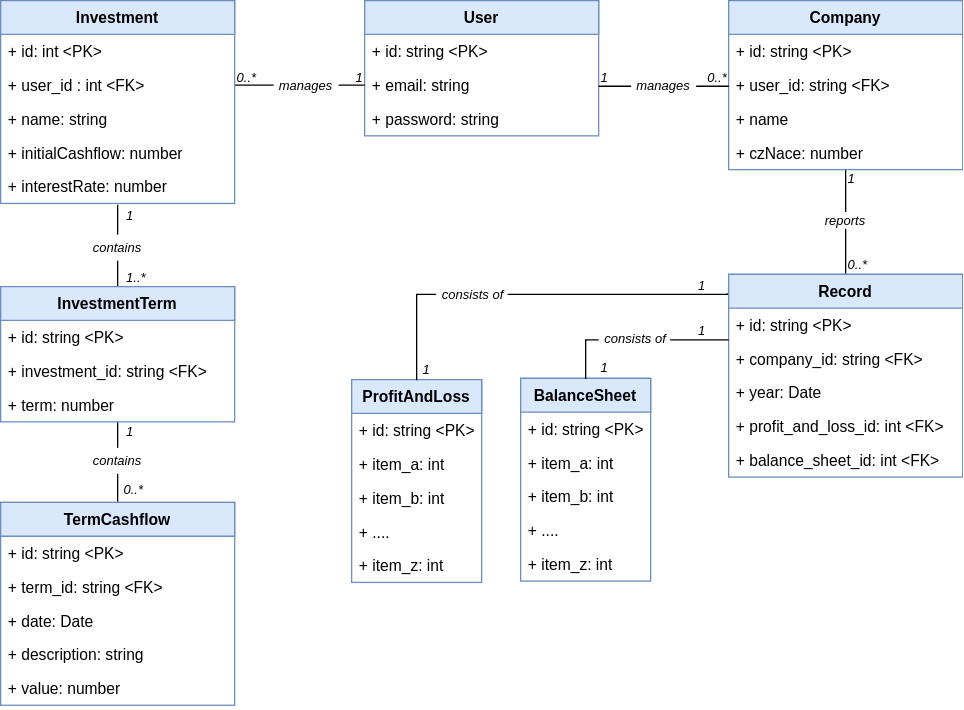
\includegraphics[width=14cm]{img/erd.png}
  \caption{ERD na fyzické úrovni}
\end{figure}

Dále bude server obsluhovat požadavky klienta. Vzhledem k~tomu, že je nástroj koncipován jako SPA (single page application), ke stažení veškerého kódu aplikace ke klientovi bude sloužit jeden jediný endpoint. Klient tak bude moci s~nástrojem pracovat bez dodatečného volání serveru, vyjma operací nad daty, jejichž uložiště ja na serveru. Server bude dále zpřístupňovat rozhraní pro CRUD operace nad těmito daty.

Zda se budou výpočty provádět na straně serveru nebo klienta se rozhodne až při implementaci a~testování. Preferovaný je výpočet na straně klienta, při většině metod analýzy se neprovádějí náročné výpočty a~objem zpracovávaných dat je relativně malý. Přesto je však potřeba dbát na to, aby zátež na klientovi nebyla znát. 



%-----
\subsection{Knihovny a~technologie}
K~implementaci bude použita kombinace programovacích, skriptovacích, značkovacích a~dotazovacích jazyků. Pro klientskou část jsou to HTML, CSS a~Javascript (přesněji TypeScript). Kód serveru bude v~jazyce PHP s~připojením na MySQL databázi.


\subsubsection{React}
React je populární frontendová knihovna v~jazyce JavaScript vyvíjená společností Facebook. Jejím jediným cílem je tvorba uživatelského rozhraní pomocí komponent, jejichž kód je zapsán deklarativně -- spíše definujeme, co se má udělat (jak má komponenta vypadat) a~ne jak se to má udělat (to za nás řeší životní cyklus komponent). Při změně modelu, který je uložen v~JavaScriptu, React na základě definice komponent pozná, které komponenty (a na pozadí tedy i uzly DOM) to ovlivní, a~překreslí pouze ty. Velkou výhodou je tedy oddělení modelu od prezentační vrstvy (v~případě jQuery je model uložen přímo v~HTML) se současným použitím deklarativního zápisu.

Systém komponent nás kompletně odstíní od manipulace s~DOM, což bývá v~případě komplexních UI, i s~pomocí jQuery, velmi nepohodlné. Aplikace manipulující přímo s~DOM jsou také velmi náročné na údržbu (změna na jednom místě vede k~změnám na mnoha jiných místech) a~její části hůře znovupoužitelné.


\subsubsection{Typescript}
Jedná se o~nástavbu jazyka JavaScript vyvíjenou společností Microsoft, jejíž hlavním přínosem je statické typování a~další techniky známé z~objektově orientovaného programování -- třídy (ačkoliv ty jsou podle nejnovější specifikace ECMAScript součástí samotného JavaScriptu), rozhraní, moduly a~podobně.

Jelikož se jedná o~nástavbu, lze používat i čistý JavaScript bez použítí typů, což nám umožní použít i knihovny, které jsou implementovány v~čistém JavaScriptu. Otypování kódu však zvyšuje jeho přehlednost, snižuje chybovost, otevírá nové možnosti pro vývojová prostředí (našeptávání, refaktorizace kódu) a~tím zkvalitňuje vývoj. Proto budeme vyvíjet striktně typovaný kód. 


\subsubsection{Ostatní}
\begin{itemize}
	\item Next.js -- startovní balík pro urychlení vývoje, obsahuje skripty pro spouštění, ladění a~jednoduchý deployment aplikace, importuje také všechny užitečné knihovny (routování, serverová volání, dynamické importování)
	\item Bootstrap -- sada přednastavených šablon, usnadní nám design uživatelského rozhraní
	\item Chart.js -- knihovna pro práci s~grafy
\end{itemize} 






%-----
\section{Shrnutí a~další postup}
V~dosavadním textu byly zmíněny základy finanční analýzy podniku -- její definice, praktický i teoretický význam, byla popsána také vstupní data analýzy. Dále byly zmíněny a~popsány pojmy horizontální a~vertikální analýza a~výběr těch nejzákladnějších poměrových ukazatelů spolu se vzorcem výpočtu a~popisem jejich významu. 

Ještě před návrhem vlastního programového řešení byl proveden průzkum současných možností v~této oblasti. Na jeho základě byl vypracován vlastní návrh, zohledňující přednosti i nedostatky vybraných nástrojů. Hlavním rozdílem je architektura aplikace (klient-server) a~prostředí běhu (webový prohlížeč). Tento výběr následuje trend moderních aplikací a činí nástroj dostupnější. Dalším významným rozdílem je výběr technologií, které učiní kód strukturovaným, lehce rozšiřielným, dlouhodobě udržovatelným a~vysoce znovupoužitelným. 

Při dalším postupu bude ze všeho nejdříve připraveno vývojové prostředí (devstack). To obnáší instalaci, zprovoznění a~nastavení IDE, PHP serveru, databáze, instalace správce balíčků a~balíčků samotných, vytvoření repozitáře, obstarání testovacích sad. Následně může začít implementace klienta, zcela nezávisle na implementaci serveru. Detaily implementace budou uvedeny v~této zprávě.



\chapter{Implementace}

\begin{comment}
aktiva: 
	17+16;
	15+14 +13[nazvy]+12+11+10[nazvy]

pasiva:
	17+16;
	15+14 +13[nazvy,radek_58_chybi]+12[radek_57_chybi]+11[radek_56_chybi]+10[nazvy]

vzz:
	17+16;
	15+14 +13[nazvy]+12+11+10

kms-mrp
kazdy rok nove zakony - nema smysl prizpusobovat do budoucna
proto kazdy ekon/ucetni program placeny pausalne - rocne
moznosti - parse do predem definovane struktury X parse do dane dppdp8_20XX struktury, tahani pomoci definovanych funkci
upgrade kazdy rok

tabulky aktiv/pasiv/vzz nelze stahnout ze zadneho endpointu (kontrolovano i v dotazech prohlizece) - muselo by se parsovat HTML cele stranky - nakonec vytvoren jednoduchy parser

aby vse fungovalo jak ma - prepocet nadrazenych polozek - musime znat strom - ten taky neni mozne automatizovane vytvorit

nemoznost vytvorit strom na zaklade atributu "oznaceni" - napr pasiva 2016 obsahuje B.+C. -> strom musi byt explicitne zapsan


jelikoz podle struktury tabulek MF jsou c_radku pomichana a obecne nejdou postupne za sebou, tabulku ulozime radeji jako objekt, nez pole; atributy objektu budou jednotliva cisla radku; bude se nam potom podle vykazu lepe vytahovat hodnota, nez pokazde zjistovat, jaky index v poli to je; dalsi varianta je ulozit vykaz do pole a potom pomoci funkce .find hledat prislusny radek; prvni varianta- rychlejsi, primy odkaz do objektu, jen bude nutne pomoci helperu inteligentne prekonvertovat objekt na pole, aby se dalo v sablone nad timto objektem iterovat pomoci map; js nezarucuje zachovani poradi atributu objektu - kazdy prohlizec jiny pristup, napr chrome seradi, proto je nutne v mape ulozit do array c_radku tak, jak jdou ve vykazu za sebou - array zachova poradi
mapa poslouzi i pri vytvareni prazdnych dokumentu pr vyplneni v budoucnu

vyber polozek - reknu co chci (trzby) a fce pozna, ktere polozky vytahnout podle roku
prevodova tabulka - pdf email

client side routing (react-router)
firebase config
material-ui-next

analyza vybraneho podniku + vystup nastroje


rozsireni: 
du pont analyza (pyramidove rozlozeni), cash flow
ulozeni ukazazelu odvetvi, porovnani s odvetvim
sirsi zaber mezipodnikoveho srovnani, nejen vykaz
offline rezim

\end{comment}